\appendix
\appendixpage

\section{Supplementary Real Data Analysis Results}
\label{sec:ap}

At the first replication on each of the 4 data sets, we first record the number of features discarded by each screening method at each $\lambda$ value along the path of $L=100$ values. Features discarded by SEDPP are safely discarded and features discarded by SSR are not safely discarded and require additional checks. For the adaptive hybrid rule, we use AHR\_Safe to denote the features that are safely discarded first by adaptive EDPP and AHR\_Strong to denote features that discarded afterward by adaptive SSR and require additional checks. The results are summarized in Figure \ref{fig:ap1}.

\begin{figure}[H]
    \centering
    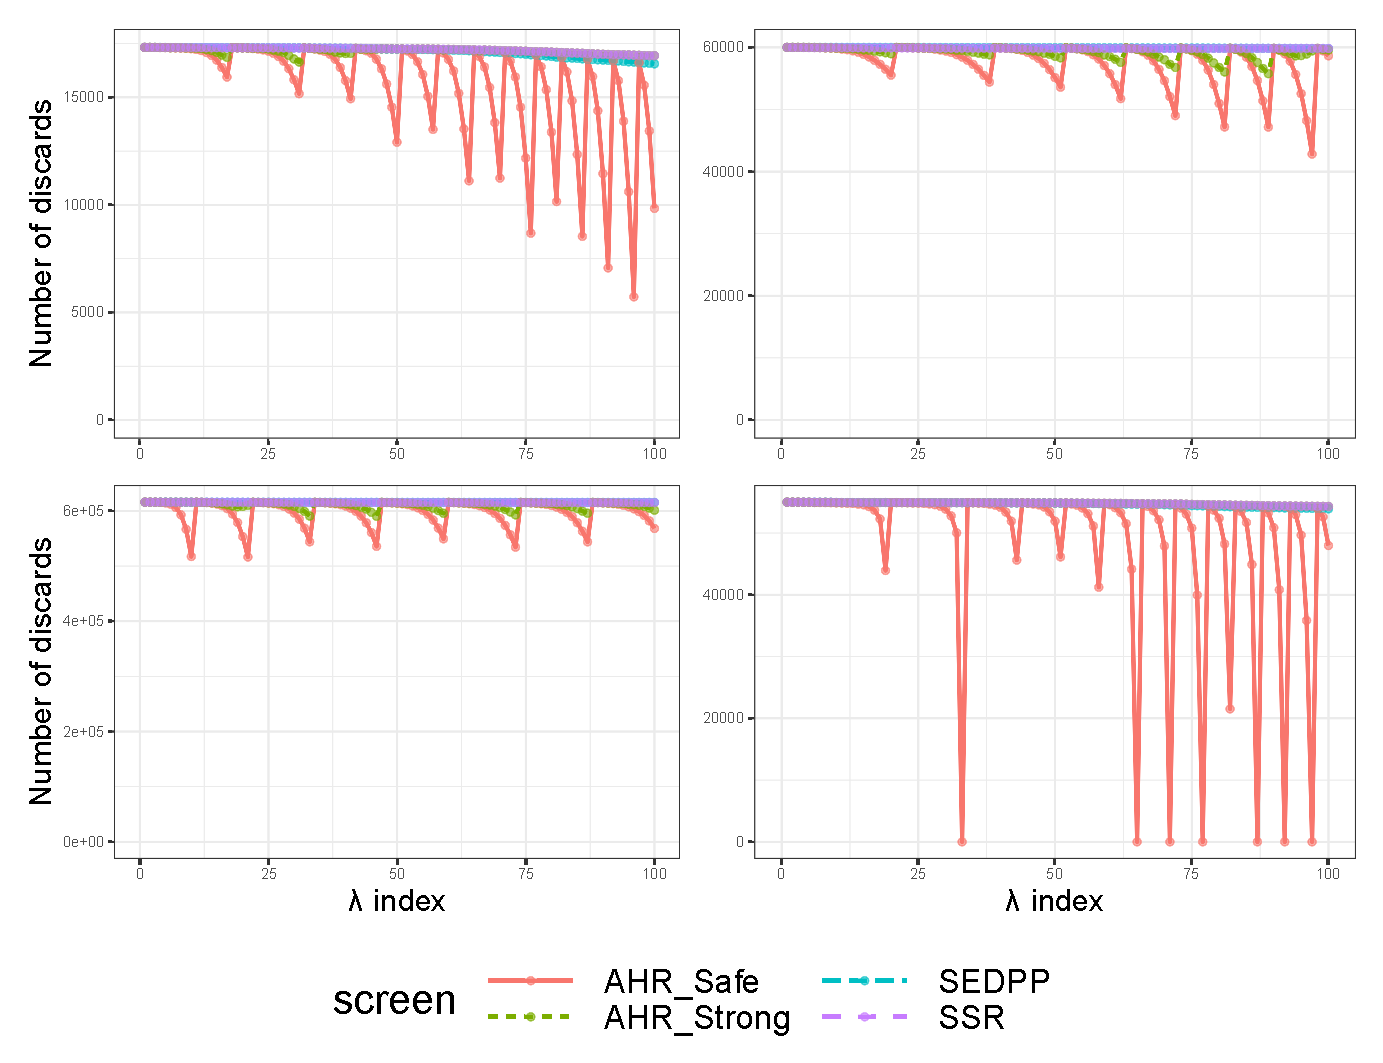
\includegraphics[width=0.82\textwidth]{app1.eps}    \caption{Comparing number of discards by screening methods for lasso model along $\lambda$ values.}
    \label{fig:ap1}
\end{figure}

Note each jump of the number of discards for AHR method indicates an update of reference because a newer reference leads to higher screening power. Our adaptive updating algorithm determines the timing of update dynamically depending on the screening performance. For all four data sets, with about only 10 updates, the adaptive hybrid screening can safely discard a great number of features at most $\lambda$ values.

Next we compare the number of rounds of KKT conditions checks and the number of KKT conditions checks on individual features, needed for AHR and SSR respectively, as shown in Table \ref{Tab:kkt1} and Table \ref{Tab:kkt2}. In a round of KKT conditions check, all features that are not discarded by the safe rule are checked, and a round a KKT conditions check potentially include a large number of KKT conditions checks on individual features. 

\begin{table}[H]
\centering
\begin{tabular}{lllll}
\toprule
Screening method & GENE & MNIST & GWAS & NYT \\
\midrule
SSR & 99 & 99 & 99 & 99 \\
AHR & 99 & 99 & 99 & 99 \\
\bottomrule
\end{tabular}
\caption{Number of rounds of KKT conditions checks required for the whole path}
\label{Tab:kkt1}
\end{table}

\begin{table}[H]
\centering
\begin{tabular}{lllll}
\toprule
Screening method & GENE & MNIST & GWAS & NYT \\
\midrule
SSR & 1,712 & 5,943 & 60,986 & 5,429 \\
AHR & 172 & 286 & 2,353 & 622 \\
\bottomrule
\end{tabular}
\caption{Number of KKT conditions checks on individual features ($\times10^3$) required for the whole path}
\label{Tab:kkt2}
\end{table}

Although a path include $L=100$ $\lambda$ values, the solution at the first value $\lambda_{0}$ is trivially $\hat{\beta}(\lambda_0)=0$ so we are essentially solving along $99$ $\lam$ values. If the strong rule does not make a violation, the minimal number of rounds of KKT conditions checks required will be $99$. In all four data sets, neither SSR nor the adaptive SSR in AHR ever makes a violation. However two methods are very different in terms of the number of KKT conditions checks on individual features, which proportionally increases the computational cost. AHR requires much less checks on individual features because the adaptive EDPP narrows down the set of features that need to be checked by a magnitude.